\documentclass[11pt]{article}
\renewcommand{\arraystretch}{1.5} % Default value: 1
\usepackage{sectsty}
\allsectionsfont{\color{blue}\fontfamily{lmss}\selectfont}
\usepackage{fontspec}
\setmainfont{XCharter}

\usepackage{listings}

\lstset{
basicstyle=\small\ttfamily,
tabsize=8,
columns=flexible,
breaklines=true,
frame=tb,
rulecolor=\color[rgb]{0.8,0.8,0.7},
backgroundcolor=\color[rgb]{1,1,0.91},
postbreak=\raisebox{0ex}[0ex][0ex]{\ensuremath{\color{red}\hookrightarrow\space}}
}
\usepackage{fontawesome}


\usepackage{mdframed}
\newmdenv[
  backgroundcolor=gray,
  fontcolor=white,
  nobreak=true,
]{terminalinput}



\usepackage{parskip}


    \usepackage[breakable]{tcolorbox}
    \usepackage{parskip} % Stop auto-indenting (to mimic markdown behaviour)

    \usepackage{iftex}
    \ifPDFTeX
    	\usepackage[T1]{fontenc}
    	\usepackage{mathpazo}
    \else
    	\usepackage{fontspec}
    \fi

    % Basic figure setup, for now with no caption control since it's done
    % automatically by Pandoc (which extracts ![](path) syntax from Markdown).
    \usepackage{graphicx}
    % Maintain compatibility with old templates. Remove in nbconvert 6.0
    \let\Oldincludegraphics\includegraphics
    % Ensure that by default, figures have no caption (until we provide a
    % proper Figure object with a Caption API and a way to capture that
    % in the conversion process - todo).
    \usepackage{caption}
    \DeclareCaptionFormat{nocaption}{}
    \captionsetup{labelformat=nolabel, textfont=bf}

    \usepackage{float}
    \floatplacement{figure}{H} % forces figures to be placed at the correct location
    \usepackage{xcolor} % Allow colors to be defined
    \usepackage{enumerate} % Needed for markdown enumerations to work
    \usepackage{geometry} % Used to adjust the document margins
    \usepackage{amsmath} % Equations
    \usepackage{amssymb} % Equations
    \usepackage{textcomp} % defines textquotesingle
    % Hack from http://tex.stackexchange.com/a/47451/13684:
    \AtBeginDocument{%
        \def\PYZsq{\textquotesingle}% Upright quotes in Pygmentized code
    }
    \usepackage{upquote} % Upright quotes for verbatim code
    \usepackage{eurosym} % defines \euro
    \usepackage[mathletters]{ucs} % Extended unicode (utf-8) support
    \usepackage{fancyvrb} % verbatim replacement that allows latex
    \usepackage{grffile} % extends the file name processing of package graphics
                         % to support a larger range
    \makeatletter % fix for old versions of grffile with XeLaTeX
    \@ifpackagelater{grffile}{2019/11/01}
    {
      % Do nothing on new versions
    }
    {
      \def\Gread@@xetex#1{%
        \IfFileExists{"\Gin@base".bb}%
        {\Gread@eps{\Gin@base.bb}}%
        {\Gread@@xetex@aux#1}%
      }
    }
    \makeatother
    \usepackage[Export]{adjustbox} % Used to constrain images to a maximum size
    \adjustboxset{max size={0.9\linewidth}{0.9\paperheight}}

    % The hyperref package gives us a pdf with properly built
    % internal navigation ('pdf bookmarks' for the table of contents,
    % internal cross-reference links, web links for URLs, etc.)
    \usepackage{hyperref}
    % The default LaTeX title has an obnoxious amount of whitespace. By default,
    % titling removes some of it. It also provides customization options.
    \usepackage{titling}
    \usepackage{longtable} % longtable support required by pandoc >1.10
    \usepackage{booktabs}  % table support for pandoc > 1.12.2
    \usepackage[inline]{enumitem} % IRkernel/repr support (it uses the enumerate* environment)
    \usepackage[normalem]{ulem} % ulem is needed to support strikethroughs (\sout)
                                % normalem makes italics be italics, not underlines
    \usepackage{mathrsfs}



    % Colors for the hyperref package
    \definecolor{urlcolor}{rgb}{0,.145,.698}
    \definecolor{linkcolor}{rgb}{.71,0.21,0.01}
    \definecolor{citecolor}{rgb}{.12,.54,.11}

    % ANSI colors
    \definecolor{ansi-black}{HTML}{3E424D}
    \definecolor{ansi-black-intense}{HTML}{282C36}
    \definecolor{ansi-red}{HTML}{E75C58}
    \definecolor{ansi-red-intense}{HTML}{B22B31}
    \definecolor{ansi-green}{HTML}{00A250}
    \definecolor{ansi-green-intense}{HTML}{007427}
    \definecolor{ansi-yellow}{HTML}{DDB62B}
    \definecolor{ansi-yellow-intense}{HTML}{B27D12}
    \definecolor{ansi-blue}{HTML}{208FFB}
    \definecolor{ansi-blue-intense}{HTML}{0065CA}
    \definecolor{ansi-magenta}{HTML}{D160C4}
    \definecolor{ansi-magenta-intense}{HTML}{A03196}
    \definecolor{ansi-cyan}{HTML}{60C6C8}
    \definecolor{ansi-cyan-intense}{HTML}{258F8F}
    \definecolor{ansi-white}{HTML}{C5C1B4}
    \definecolor{ansi-white-intense}{HTML}{A1A6B2}
    \definecolor{ansi-default-inverse-fg}{HTML}{FFFFFF}
    \definecolor{ansi-default-inverse-bg}{HTML}{000000}

    % common color for the border for error outputs.
    \definecolor{outerrorbackground}{HTML}{FFDFDF}

    % commands and environments needed by pandoc snippets
    % extracted from the output of `pandoc -s`
    \providecommand{\tightlist}{%
      \setlength{\itemsep}{0pt}\setlength{\parskip}{0pt}}
    \DefineVerbatimEnvironment{Highlighting}{Verbatim}{commandchars=\\\{\}}
    % Add ',fontsize=\small' for more characters per line
    \newenvironment{Shaded}{}{}
    \newcommand{\KeywordTok}[1]{\textcolor[rgb]{0.00,0.44,0.13}{\textbf{{#1}}}}
    \newcommand{\DataTypeTok}[1]{\textcolor[rgb]{0.56,0.13,0.00}{{#1}}}
    \newcommand{\DecValTok}[1]{\textcolor[rgb]{0.25,0.63,0.44}{{#1}}}
    \newcommand{\BaseNTok}[1]{\textcolor[rgb]{0.25,0.63,0.44}{{#1}}}
    \newcommand{\FloatTok}[1]{\textcolor[rgb]{0.25,0.63,0.44}{{#1}}}
    \newcommand{\CharTok}[1]{\textcolor[rgb]{0.25,0.44,0.63}{{#1}}}
    \newcommand{\StringTok}[1]{\textcolor[rgb]{0.25,0.44,0.63}{{#1}}}
    \newcommand{\CommentTok}[1]{\textcolor[rgb]{0.38,0.63,0.69}{\textit{{#1}}}}
    \newcommand{\OtherTok}[1]{\textcolor[rgb]{0.00,0.44,0.13}{{#1}}}
    \newcommand{\AlertTok}[1]{\textcolor[rgb]{1.00,0.00,0.00}{\textbf{{#1}}}}
    \newcommand{\FunctionTok}[1]{\textcolor[rgb]{0.02,0.16,0.49}{{#1}}}
    \newcommand{\RegionMarkerTok}[1]{{#1}}
    \newcommand{\ErrorTok}[1]{\textcolor[rgb]{1.00,0.00,0.00}{\textbf{{#1}}}}
    \newcommand{\NormalTok}[1]{{#1}}

    % Additional commands for more recent versions of Pandoc
    \newcommand{\ConstantTok}[1]{\textcolor[rgb]{0.53,0.00,0.00}{{#1}}}
    \newcommand{\SpecialCharTok}[1]{\textcolor[rgb]{0.25,0.44,0.63}{{#1}}}
    \newcommand{\VerbatimStringTok}[1]{\textcolor[rgb]{0.25,0.44,0.63}{{#1}}}
    \newcommand{\SpecialStringTok}[1]{\textcolor[rgb]{0.73,0.40,0.53}{{#1}}}
    \newcommand{\ImportTok}[1]{{#1}}
    \newcommand{\DocumentationTok}[1]{\textcolor[rgb]{0.73,0.13,0.13}{\textit{{#1}}}}
    \newcommand{\AnnotationTok}[1]{\textcolor[rgb]{0.38,0.63,0.69}{\textbf{\textit{{#1}}}}}
    \newcommand{\CommentVarTok}[1]{\textcolor[rgb]{0.38,0.63,0.69}{\textbf{\textit{{#1}}}}}
    \newcommand{\VariableTok}[1]{\textcolor[rgb]{0.10,0.09,0.49}{{#1}}}
    \newcommand{\ControlFlowTok}[1]{\textcolor[rgb]{0.00,0.44,0.13}{\textbf{{#1}}}}
    \newcommand{\OperatorTok}[1]{\textcolor[rgb]{0.40,0.40,0.40}{{#1}}}
    \newcommand{\BuiltInTok}[1]{{#1}}
    \newcommand{\ExtensionTok}[1]{{#1}}
    \newcommand{\PreprocessorTok}[1]{\textcolor[rgb]{0.74,0.48,0.00}{{#1}}}
    \newcommand{\AttributeTok}[1]{\textcolor[rgb]{0.49,0.56,0.16}{{#1}}}
    \newcommand{\InformationTok}[1]{\textcolor[rgb]{0.38,0.63,0.69}{\textbf{\textit{{#1}}}}}
    \newcommand{\WarningTok}[1]{\textcolor[rgb]{0.38,0.63,0.69}{\textbf{\textit{{#1}}}}}


    % Define a nice break command that doesn't care if a line doesn't already
    % exist.
    \def\br{\hspace*{\fill} \\* }
    % Math Jax compatibility definitions
    \def\gt{>}
    \def\lt{<}
    \let\Oldtex\TeX
    \let\Oldlatex\LaTeX
    \renewcommand{\TeX}{\textrm{\Oldtex}}
    \renewcommand{\LaTeX}{\textrm{\Oldlatex}}
    % Document parameters
    % Document title
    \title{index}





% Pygments definitions
\makeatletter
\def\PY@reset{\let\PY@it=\relax \let\PY@bf=\relax%
    \let\PY@ul=\relax \let\PY@tc=\relax%
    \let\PY@bc=\relax \let\PY@ff=\relax}
\def\PY@tok#1{\csname PY@tok@#1\endcsname}
\def\PY@toks#1+{\ifx\relax#1\empty\else%
    \PY@tok{#1}\expandafter\PY@toks\fi}
\def\PY@do#1{\PY@bc{\PY@tc{\PY@ul{%
    \PY@it{\PY@bf{\PY@ff{#1}}}}}}}
\def\PY#1#2{\PY@reset\PY@toks#1+\relax+\PY@do{#2}}

\expandafter\def\csname PY@tok@w\endcsname{\def\PY@tc##1{\textcolor[rgb]{0.73,0.73,0.73}{##1}}}
\expandafter\def\csname PY@tok@c\endcsname{\let\PY@it=\textit\def\PY@tc##1{\textcolor[rgb]{0.25,0.50,0.50}{##1}}}
\expandafter\def\csname PY@tok@cp\endcsname{\def\PY@tc##1{\textcolor[rgb]{0.74,0.48,0.00}{##1}}}
\expandafter\def\csname PY@tok@k\endcsname{\let\PY@bf=\textbf\def\PY@tc##1{\textcolor[rgb]{0.00,0.50,0.00}{##1}}}
\expandafter\def\csname PY@tok@kp\endcsname{\def\PY@tc##1{\textcolor[rgb]{0.00,0.50,0.00}{##1}}}
\expandafter\def\csname PY@tok@kt\endcsname{\def\PY@tc##1{\textcolor[rgb]{0.69,0.00,0.25}{##1}}}
\expandafter\def\csname PY@tok@o\endcsname{\def\PY@tc##1{\textcolor[rgb]{0.40,0.40,0.40}{##1}}}
\expandafter\def\csname PY@tok@ow\endcsname{\let\PY@bf=\textbf\def\PY@tc##1{\textcolor[rgb]{0.67,0.13,1.00}{##1}}}
\expandafter\def\csname PY@tok@nb\endcsname{\def\PY@tc##1{\textcolor[rgb]{0.00,0.50,0.00}{##1}}}
\expandafter\def\csname PY@tok@nf\endcsname{\def\PY@tc##1{\textcolor[rgb]{0.00,0.00,1.00}{##1}}}
\expandafter\def\csname PY@tok@nc\endcsname{\let\PY@bf=\textbf\def\PY@tc##1{\textcolor[rgb]{0.00,0.00,1.00}{##1}}}
\expandafter\def\csname PY@tok@nn\endcsname{\let\PY@bf=\textbf\def\PY@tc##1{\textcolor[rgb]{0.00,0.00,1.00}{##1}}}
\expandafter\def\csname PY@tok@ne\endcsname{\let\PY@bf=\textbf\def\PY@tc##1{\textcolor[rgb]{0.82,0.25,0.23}{##1}}}
\expandafter\def\csname PY@tok@nv\endcsname{\def\PY@tc##1{\textcolor[rgb]{0.10,0.09,0.49}{##1}}}
\expandafter\def\csname PY@tok@no\endcsname{\def\PY@tc##1{\textcolor[rgb]{0.53,0.00,0.00}{##1}}}
\expandafter\def\csname PY@tok@nl\endcsname{\def\PY@tc##1{\textcolor[rgb]{0.63,0.63,0.00}{##1}}}
\expandafter\def\csname PY@tok@ni\endcsname{\let\PY@bf=\textbf\def\PY@tc##1{\textcolor[rgb]{0.60,0.60,0.60}{##1}}}
\expandafter\def\csname PY@tok@na\endcsname{\def\PY@tc##1{\textcolor[rgb]{0.49,0.56,0.16}{##1}}}
\expandafter\def\csname PY@tok@nt\endcsname{\let\PY@bf=\textbf\def\PY@tc##1{\textcolor[rgb]{0.00,0.50,0.00}{##1}}}
\expandafter\def\csname PY@tok@nd\endcsname{\def\PY@tc##1{\textcolor[rgb]{0.67,0.13,1.00}{##1}}}
\expandafter\def\csname PY@tok@s\endcsname{\def\PY@tc##1{\textcolor[rgb]{0.73,0.13,0.13}{##1}}}
\expandafter\def\csname PY@tok@sd\endcsname{\let\PY@it=\textit\def\PY@tc##1{\textcolor[rgb]{0.73,0.13,0.13}{##1}}}
\expandafter\def\csname PY@tok@si\endcsname{\let\PY@bf=\textbf\def\PY@tc##1{\textcolor[rgb]{0.73,0.40,0.53}{##1}}}
\expandafter\def\csname PY@tok@se\endcsname{\let\PY@bf=\textbf\def\PY@tc##1{\textcolor[rgb]{0.73,0.40,0.13}{##1}}}
\expandafter\def\csname PY@tok@sr\endcsname{\def\PY@tc##1{\textcolor[rgb]{0.73,0.40,0.53}{##1}}}
\expandafter\def\csname PY@tok@ss\endcsname{\def\PY@tc##1{\textcolor[rgb]{0.10,0.09,0.49}{##1}}}
\expandafter\def\csname PY@tok@sx\endcsname{\def\PY@tc##1{\textcolor[rgb]{0.00,0.50,0.00}{##1}}}
\expandafter\def\csname PY@tok@m\endcsname{\def\PY@tc##1{\textcolor[rgb]{0.40,0.40,0.40}{##1}}}
\expandafter\def\csname PY@tok@gh\endcsname{\let\PY@bf=\textbf\def\PY@tc##1{\textcolor[rgb]{0.00,0.00,0.50}{##1}}}
\expandafter\def\csname PY@tok@gu\endcsname{\let\PY@bf=\textbf\def\PY@tc##1{\textcolor[rgb]{0.50,0.00,0.50}{##1}}}
\expandafter\def\csname PY@tok@gd\endcsname{\def\PY@tc##1{\textcolor[rgb]{0.63,0.00,0.00}{##1}}}
\expandafter\def\csname PY@tok@gi\endcsname{\def\PY@tc##1{\textcolor[rgb]{0.00,0.63,0.00}{##1}}}
\expandafter\def\csname PY@tok@gr\endcsname{\def\PY@tc##1{\textcolor[rgb]{1.00,0.00,0.00}{##1}}}
\expandafter\def\csname PY@tok@ge\endcsname{\let\PY@it=\textit}
\expandafter\def\csname PY@tok@gs\endcsname{\let\PY@bf=\textbf}
\expandafter\def\csname PY@tok@gp\endcsname{\let\PY@bf=\textbf\def\PY@tc##1{\textcolor[rgb]{0.00,0.00,0.50}{##1}}}
\expandafter\def\csname PY@tok@go\endcsname{\def\PY@tc##1{\textcolor[rgb]{0.53,0.53,0.53}{##1}}}
\expandafter\def\csname PY@tok@gt\endcsname{\def\PY@tc##1{\textcolor[rgb]{0.00,0.27,0.87}{##1}}}
\expandafter\def\csname PY@tok@err\endcsname{\def\PY@bc##1{\setlength{\fboxsep}{0pt}\fcolorbox[rgb]{1.00,0.00,0.00}{1,1,1}{\strut ##1}}}
\expandafter\def\csname PY@tok@kc\endcsname{\let\PY@bf=\textbf\def\PY@tc##1{\textcolor[rgb]{0.00,0.50,0.00}{##1}}}
\expandafter\def\csname PY@tok@kd\endcsname{\let\PY@bf=\textbf\def\PY@tc##1{\textcolor[rgb]{0.00,0.50,0.00}{##1}}}
\expandafter\def\csname PY@tok@kn\endcsname{\let\PY@bf=\textbf\def\PY@tc##1{\textcolor[rgb]{0.00,0.50,0.00}{##1}}}
\expandafter\def\csname PY@tok@kr\endcsname{\let\PY@bf=\textbf\def\PY@tc##1{\textcolor[rgb]{0.00,0.50,0.00}{##1}}}
\expandafter\def\csname PY@tok@bp\endcsname{\def\PY@tc##1{\textcolor[rgb]{0.00,0.50,0.00}{##1}}}
\expandafter\def\csname PY@tok@fm\endcsname{\def\PY@tc##1{\textcolor[rgb]{0.00,0.00,1.00}{##1}}}
\expandafter\def\csname PY@tok@vc\endcsname{\def\PY@tc##1{\textcolor[rgb]{0.10,0.09,0.49}{##1}}}
\expandafter\def\csname PY@tok@vg\endcsname{\def\PY@tc##1{\textcolor[rgb]{0.10,0.09,0.49}{##1}}}
\expandafter\def\csname PY@tok@vi\endcsname{\def\PY@tc##1{\textcolor[rgb]{0.10,0.09,0.49}{##1}}}
\expandafter\def\csname PY@tok@vm\endcsname{\def\PY@tc##1{\textcolor[rgb]{0.10,0.09,0.49}{##1}}}
\expandafter\def\csname PY@tok@sa\endcsname{\def\PY@tc##1{\textcolor[rgb]{0.73,0.13,0.13}{##1}}}
\expandafter\def\csname PY@tok@sb\endcsname{\def\PY@tc##1{\textcolor[rgb]{0.73,0.13,0.13}{##1}}}
\expandafter\def\csname PY@tok@sc\endcsname{\def\PY@tc##1{\textcolor[rgb]{0.73,0.13,0.13}{##1}}}
\expandafter\def\csname PY@tok@dl\endcsname{\def\PY@tc##1{\textcolor[rgb]{0.73,0.13,0.13}{##1}}}
\expandafter\def\csname PY@tok@s2\endcsname{\def\PY@tc##1{\textcolor[rgb]{0.73,0.13,0.13}{##1}}}
\expandafter\def\csname PY@tok@sh\endcsname{\def\PY@tc##1{\textcolor[rgb]{0.73,0.13,0.13}{##1}}}
\expandafter\def\csname PY@tok@s1\endcsname{\def\PY@tc##1{\textcolor[rgb]{0.73,0.13,0.13}{##1}}}
\expandafter\def\csname PY@tok@mb\endcsname{\def\PY@tc##1{\textcolor[rgb]{0.40,0.40,0.40}{##1}}}
\expandafter\def\csname PY@tok@mf\endcsname{\def\PY@tc##1{\textcolor[rgb]{0.40,0.40,0.40}{##1}}}
\expandafter\def\csname PY@tok@mh\endcsname{\def\PY@tc##1{\textcolor[rgb]{0.40,0.40,0.40}{##1}}}
\expandafter\def\csname PY@tok@mi\endcsname{\def\PY@tc##1{\textcolor[rgb]{0.40,0.40,0.40}{##1}}}
\expandafter\def\csname PY@tok@il\endcsname{\def\PY@tc##1{\textcolor[rgb]{0.40,0.40,0.40}{##1}}}
\expandafter\def\csname PY@tok@mo\endcsname{\def\PY@tc##1{\textcolor[rgb]{0.40,0.40,0.40}{##1}}}
\expandafter\def\csname PY@tok@ch\endcsname{\let\PY@it=\textit\def\PY@tc##1{\textcolor[rgb]{0.25,0.50,0.50}{##1}}}
\expandafter\def\csname PY@tok@cm\endcsname{\let\PY@it=\textit\def\PY@tc##1{\textcolor[rgb]{0.25,0.50,0.50}{##1}}}
\expandafter\def\csname PY@tok@cpf\endcsname{\let\PY@it=\textit\def\PY@tc##1{\textcolor[rgb]{0.25,0.50,0.50}{##1}}}
\expandafter\def\csname PY@tok@c1\endcsname{\let\PY@it=\textit\def\PY@tc##1{\textcolor[rgb]{0.25,0.50,0.50}{##1}}}
\expandafter\def\csname PY@tok@cs\endcsname{\let\PY@it=\textit\def\PY@tc##1{\textcolor[rgb]{0.25,0.50,0.50}{##1}}}

\def\PYZbs{\char`\\}
\def\PYZus{\char`\_}
\def\PYZob{\char`\{}
\def\PYZcb{\char`\}}
\def\PYZca{\char`\^}
\def\PYZam{\char`\&}
\def\PYZlt{\char`\<}
\def\PYZgt{\char`\>}
\def\PYZsh{\char`\#}
\def\PYZpc{\char`\%}
\def\PYZdl{\char`\$}
\def\PYZhy{\char`\-}
\def\PYZsq{\char`\'}
\def\PYZdq{\char`\"}
\def\PYZti{\char`\~}
% for compatibility with earlier versions
\def\PYZat{@}
\def\PYZlb{[}
\def\PYZrb{]}
\makeatother


    % For linebreaks inside Verbatim environment from package fancyvrb.
    \makeatletter
        \newbox\Wrappedcontinuationbox
        \newbox\Wrappedvisiblespacebox
        \newcommand*\Wrappedvisiblespace {\textcolor{red}{\textvisiblespace}}
        \newcommand*\Wrappedcontinuationsymbol {\textcolor{red}{\llap{\tiny$\m@th\hookrightarrow$}}}
        \newcommand*\Wrappedcontinuationindent {3ex }
        \newcommand*\Wrappedafterbreak {\kern\Wrappedcontinuationindent\copy\Wrappedcontinuationbox}
        % Take advantage of the already applied Pygments mark-up to insert
        % potential linebreaks for TeX processing.
        %        {, <, #, %, $, ' and ": go to next line.
        %        _, }, ^, &, >, - and ~: stay at end of broken line.
        % Use of \textquotesingle for straight quote.
        \newcommand*\Wrappedbreaksatspecials {%
            \def\PYGZus{\discretionary{\char`\_}{\Wrappedafterbreak}{\char`\_}}%
            \def\PYGZob{\discretionary{}{\Wrappedafterbreak\char`\{}{\char`\{}}%
            \def\PYGZcb{\discretionary{\char`\}}{\Wrappedafterbreak}{\char`\}}}%
            \def\PYGZca{\discretionary{\char`\^}{\Wrappedafterbreak}{\char`\^}}%
            \def\PYGZam{\discretionary{\char`\&}{\Wrappedafterbreak}{\char`\&}}%
            \def\PYGZlt{\discretionary{}{\Wrappedafterbreak\char`\<}{\char`\<}}%
            \def\PYGZgt{\discretionary{\char`\>}{\Wrappedafterbreak}{\char`\>}}%
            \def\PYGZsh{\discretionary{}{\Wrappedafterbreak\char`\#}{\char`\#}}%
            \def\PYGZpc{\discretionary{}{\Wrappedafterbreak\char`\%}{\char`\%}}%
            \def\PYGZdl{\discretionary{}{\Wrappedafterbreak\char`\$}{\char`\$}}%
            \def\PYGZhy{\discretionary{\char`\-}{\Wrappedafterbreak}{\char`\-}}%
            \def\PYGZsq{\discretionary{}{\Wrappedafterbreak\textquotesingle}{\textquotesingle}}%
            \def\PYGZdq{\discretionary{}{\Wrappedafterbreak\char`\"}{\char`\"}}%
            \def\PYGZti{\discretionary{\char`\~}{\Wrappedafterbreak}{\char`\~}}%
        }
        % Some characters . , ; ? ! / are not pygmentized.
        % This macro makes them "active" and they will insert potential linebreaks
        \newcommand*\Wrappedbreaksatpunct {%
            \lccode`\~`\.\lowercase{\def~}{\discretionary{\hbox{\char`\.}}{\Wrappedafterbreak}{\hbox{\char`\.}}}%
            \lccode`\~`\,\lowercase{\def~}{\discretionary{\hbox{\char`\,}}{\Wrappedafterbreak}{\hbox{\char`\,}}}%
            \lccode`\~`\;\lowercase{\def~}{\discretionary{\hbox{\char`\;}}{\Wrappedafterbreak}{\hbox{\char`\;}}}%
            \lccode`\~`\:\lowercase{\def~}{\discretionary{\hbox{\char`\:}}{\Wrappedafterbreak}{\hbox{\char`\:}}}%
            \lccode`\~`\?\lowercase{\def~}{\discretionary{\hbox{\char`\?}}{\Wrappedafterbreak}{\hbox{\char`\?}}}%
            \lccode`\~`\!\lowercase{\def~}{\discretionary{\hbox{\char`\!}}{\Wrappedafterbreak}{\hbox{\char`\!}}}%
            \lccode`\~`\/\lowercase{\def~}{\discretionary{\hbox{\char`\/}}{\Wrappedafterbreak}{\hbox{\char`\/}}}%
            \catcode`\.\active
            \catcode`\,\active
            \catcode`\;\active
            \catcode`\:\active
            \catcode`\?\active
            \catcode`\!\active
            \catcode`\/\active
            \lccode`\~`\~
        }
    \makeatother

    \let\OriginalVerbatim=\Verbatim
    \makeatletter
    \renewcommand{\Verbatim}[1][1]{%
        %\parskip\z@skip
        \sbox\Wrappedcontinuationbox {\Wrappedcontinuationsymbol}%
        \sbox\Wrappedvisiblespacebox {\FV@SetupFont\Wrappedvisiblespace}%
        \def\FancyVerbFormatLine ##1{\hsize\linewidth
            \vtop{\raggedright\hyphenpenalty\z@\exhyphenpenalty\z@
                \doublehyphendemerits\z@\finalhyphendemerits\z@
                \strut ##1\strut}%
        }%
        % If the linebreak is at a space, the latter will be displayed as visible
        % space at end of first line, and a continuation symbol starts next line.
        % Stretch/shrink are however usually zero for typewriter font.
        \def\FV@Space {%
            \nobreak\hskip\z@ plus\fontdimen3\font minus\fontdimen4\font
            \discretionary{\copy\Wrappedvisiblespacebox}{\Wrappedafterbreak}
            {\kern\fontdimen2\font}%
        }%

        % Allow breaks at special characters using \PYG... macros.
        \Wrappedbreaksatspecials
        % Breaks at punctuation characters . , ; ? ! and / need catcode=\active
        \OriginalVerbatim[#1,codes*=\Wrappedbreaksatpunct]%
    }
    \makeatother

    % Exact colors from NB
    \definecolor{incolor}{HTML}{303F9F}
    \definecolor{outcolor}{HTML}{D84315}
    \definecolor{cellborder}{HTML}{CFCFCF}
    \definecolor{cellbackground}{HTML}{F7F7F7}

    % prompt
    \makeatletter
    \newcommand{\boxspacing}{\kern\kvtcb@left@rule\kern\kvtcb@boxsep}
    \makeatother
    \newcommand{\prompt}[4]{

        {\ttfamily\llap{{\color{blue}\LARGE\faKeyboardO\hspace{3pt}#4}}\vspace{-\baselineskip}}
    }



    % Prevent overflowing lines due to hard-to-break entities
    \sloppy
    % Setup hyperref package
    \hypersetup{
      breaklinks=true,  % so long urls are correctly broken across lines
      colorlinks=true,
      urlcolor=urlcolor,
      linkcolor=linkcolor,
      citecolor=citecolor,
      }
    % Slightly bigger margins than the latex defaults

    \geometry{verbose,tmargin=1in,bmargin=1in,lmargin=1in,rmargin=1in}



\renewcommand{\PY}[2]{{#2}}
\usepackage{fancyhdr}
\pagestyle{fancy}
\rhead{\color{gray}\sf\small\rightmark}
\lhead{\nouppercase{\color{gray}\sf\small\leftmark}}
\cfoot{\color{gray}\sf\thepage}
\renewcommand{\footrulewidth}{1pt}
\begin{document}





    \hypertarget{variant-calling}{%
\section{Variant Calling}\label{variant-calling}}

\hypertarget{introduction}{%
\subsection{Introduction}\label{introduction}}

Variant calling is the process of identifying differences between the
reference genome and the samples that have been sequenced. These
differences can be single nucleotide polymorphisms (SNPs),
multi-nucleotide polymorphisms (MNPs) or small insertions and deletions
(indels) and examples of each of these are shown below.

    \begin{figure}[!h]
\centering
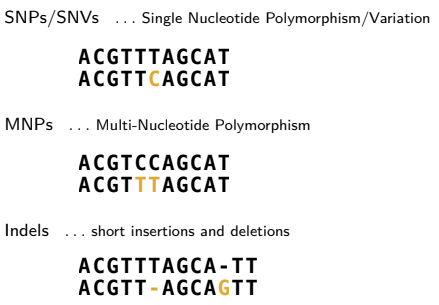
\includegraphics{images/snps-and-indels.png}
\caption{SNPs and small insertions and deletions}
\end{figure}

    \hypertarget{learning-outcomes}{%
\subsection{Learning outcomes}\label{learning-outcomes}}

On completion of the tutorial, you can expect to be able to:

\begin{itemize}
\tightlist
\item
  Perform variant calling (SNPs and indels) using standard tools
\item
  Assess the quality/confidence of a variant call
\item
  Filter variant calls to remove low quality/confidence calls
\item
  Perform variant calling across multiple samples
\item
  Visualise variants using standard tools
\item
  Annotate variants with consequence calls
\end{itemize}

\hypertarget{tutorial-sections}{%
\subsection{Tutorial sections}\label{tutorial-sections}}

This tutorial comprises the following sections:\\
1. \href{variant-calling.ipynb}{Performing variant calling} 2.
\href{filtering.ipynb}{Filtering variants} 3.
\href{multi-sample-calling.ipynb}{Multi-sample variant calling} 4.
\href{visualisation.ipynb}{Visualising variants}

There is also an additional (optional) section: 5.
\href{annotation.ipynb}{Variant annotation}

\hypertarget{authors}{%
\subsection{Authors}\label{authors}}

This tutorial was written by
\href{https://github.com/jacquikeane}{Jacqui Keane} based on material
from \href{https://github.com/tk2}{Thomas Keane} and
\href{https://github.com/pd3}{Petr Danecek}.

\hypertarget{running-the-commands-from-this-tutorial}{%
\subsection{Running the commands from this
tutorial}\label{running-the-commands-from-this-tutorial}}

You can follow this tutorial by typing all the commands you see into a
terminal window. This is similar to the ``Command Prompt'' window on MS
Windows systems, which allows the user to type DOS commands to manage
files.

To get started, open a new terminal on your computer and type the
command below:

    \begin{tcolorbox}[breakable, size=fbox, boxrule=1pt, pad at break*=1mm,colback=cellbackground, colframe=cellborder]
\prompt{In}{incolor}{ }{\boxspacing}
\begin{Verbatim}[commandchars=\\\{\}]
\PY{n+nb}{cd} \PYZti{}/course\PYZus{}data/variant\PYZus{}calling/data
\end{Verbatim}
\end{tcolorbox}

    Now you can follow the instructions in the tutorial from here.

\hypertarget{lets-get-started}{%
\subsection{Let's get started!}\label{lets-get-started}}

This tutorial assumes that you have samtools, bcftools and IGV installed
on your computer. These are already installed on the VM you are using.
To check that these are installed, you can run the following commands:

    \begin{tcolorbox}[breakable, size=fbox, boxrule=1pt, pad at break*=1mm,colback=cellbackground, colframe=cellborder]
\prompt{In}{incolor}{ }{\boxspacing}
\begin{Verbatim}[commandchars=\\\{\}]
samtools \PYZhy{}\PYZhy{}help
\end{Verbatim}
\end{tcolorbox}

    \begin{tcolorbox}[breakable, size=fbox, boxrule=1pt, pad at break*=1mm,colback=cellbackground, colframe=cellborder]
\prompt{In}{incolor}{ }{\boxspacing}
\begin{Verbatim}[commandchars=\\\{\}]
bcftools \PYZhy{}\PYZhy{}help
\end{Verbatim}
\end{tcolorbox}

    \begin{tcolorbox}[breakable, size=fbox, boxrule=1pt, pad at break*=1mm,colback=cellbackground, colframe=cellborder]
\prompt{In}{incolor}{ }{\boxspacing}
\begin{Verbatim}[commandchars=\\\{\}]
igv
\end{Verbatim}
\end{tcolorbox}

    This should return the help message for samtools and bcftools. The final
command should launch the genome viewer IGV. You can close the IGV
software, we will use it later in this tutorial to visualise variants.

To get started with the tutorial, go to to the first section:
\href{variant-calling.ipynb}{Performing variant calling}


    % Add a bibliography block to the postdoc



\newpage





    \hypertarget{performing-variant-calling}{%
\section{Performing Variant Calling}\label{performing-variant-calling}}

When performing variant calling we need the aligned sequences in SAM,
BAM or CRAM format and the reference genome that we want to call varants
against.

First, check you are in the correct directory.

    \begin{tcolorbox}[breakable, size=fbox, boxrule=1pt, pad at break*=1mm,colback=cellbackground, colframe=cellborder]
\prompt{In}{incolor}{ }{\boxspacing}
\begin{Verbatim}[commandchars=\\\{\}]
\PY{n+nb}{pwd}
\end{Verbatim}
\end{tcolorbox}

    It should display something like:

\texttt{/home/manager/course\_data/variant\_calling/data}

    \hypertarget{assessing-the-input-data}{%
\subsection{Assessing the input data}\label{assessing-the-input-data}}

To list the files in the current directory, type

    \begin{tcolorbox}[breakable, size=fbox, boxrule=1pt, pad at break*=1mm,colback=cellbackground, colframe=cellborder]
\prompt{In}{incolor}{ }{\boxspacing}
\begin{Verbatim}[commandchars=\\\{\}]
ls \PYZhy{}lh
\end{Verbatim}
\end{tcolorbox}

    The listing shows aligned data for two mouse strains A/J and NZO
(A\_J.bam and NZO.bam) and the chromosome 19 of the mouse reference
genome (GRCm38\_68.19.fa).

    Before performing variant calling, it is important to check the quality
of the data that you will be working with. We have already seen how to
do this in the QC and Data Formats and Read Alignment sessions. The
commands would look like:

\texttt{samtools\ stats\ -r\ GRCm38\_68.19.fa\ A\_J.bam\ \textgreater{}\ A\_J.stats}

\texttt{samtools\ stats\ -r\ GRCm38\_68.19.fa\ NZO.bam\ \textgreater{}\ NZO.stats}

\texttt{plot-bamstats\ -r\ GRCm38\_68.19.fa.gc\ -p\ A\_J.graphs/\ A\_J.stats}

\texttt{plot-bamstats\ -r\ GRCm38\_68.19.fa.gc\ -p\ NZO.graphs/\ NZO.stats}

You do not need to run these QC checks on this data and for this we will
assume that QC has already been performed and the data is of good
quality.

    \hypertarget{generating-pileup}{%
\subsection{Generating pileup}\label{generating-pileup}}

The command \texttt{samtools\ mpileup} prints the read bases that align
to each position in the reference genome. Type the command:

    \begin{tcolorbox}[breakable, size=fbox, boxrule=1pt, pad at break*=1mm,colback=cellbackground, colframe=cellborder]
\prompt{In}{incolor}{ }{\boxspacing}
\begin{Verbatim}[commandchars=\\\{\}]
samtools mpileup \PYZhy{}f GRCm38\PYZus{}68.19.fa A\PYZus{}J.bam \PY{p}{|} less \PYZhy{}S
\end{Verbatim}
\end{tcolorbox}

    Each line corresponds to a position on the genome.

The columns are: chromosome, position, reference base, read depth, read
bases (dot . and comma , indicate match on the forward and on the
reverse strand; ACGTN and acgtn a mismatch on the forward and the
reverse strand) and the final column is the base qualities encoded into
characters. The caret symbol \^{} marks the start of a read, the dollar
sign \$ the end of a read, deleted bases are represented by asterisk *.

This output can be used for a simple consensus calling. One rarely needs
this type of output. Instead, for a more sophisticated variant calling
method, see the next section.

    \hypertarget{exercises}{%
\subsubsection{Exercises}\label{exercises}}

Look at the output from the \texttt{mpileup} command above and answer
the following questions.

\textbf{Q1:} What is the read depth at position 10001994? (Rather than
scrolling to the position, use the substring searching capabilities of
less: press /, then type 10001994 followed by enter to find the
position.)

\textbf{Q2:} What is the reference allele and the alternate allele at
position 10001994?

\textbf{Q3:} How many reads call the reference allele at position
10001994 and how many reads call the alternate allele at position
10001994?

    \hypertarget{generating-genotype-likelihoods-and-calling-variants}{%
\subsection{Generating genotype likelihoods and calling
variants}\label{generating-genotype-likelihoods-and-calling-variants}}

The \texttt{bcftools\ mpileup} command can be used to generate genotype
likelihoods. (Beware: the command mpileup is present in both samtools
and bcftools, but in both they do different things. While
\texttt{samtools\ mpileup} produces the text pileup output seen in the
previous exercise, \texttt{bcftools\ mpileup} generates a VCF file with
genotype likelihoods.)

Run the following command (when done, press q to quit the viewing mode):

    \begin{tcolorbox}[breakable, size=fbox, boxrule=1pt, pad at break*=1mm,colback=cellbackground, colframe=cellborder]
\prompt{In}{incolor}{ }{\boxspacing}
\begin{Verbatim}[commandchars=\\\{\}]
bcftools mpileup \PYZhy{}f GRCm38\PYZus{}68.19.fa A\PYZus{}J.bam \PY{p}{|} less \PYZhy{}S
\end{Verbatim}
\end{tcolorbox}

    This generates an intermediate output which contains genotype
likelihoods and other raw information necessary for variant calling.
This output is usually streamed directly to the caller like this

\texttt{bcftools\ mpileup\ -f\ GRCm38\_68.19.fa\ A\_J.bam\ \textbar{}\ bcftools\ call\ -m\ \textbar{}\ less\ -S}

The output above contains both variant and non-variant positions. Check
the input/output options section of the \texttt{bcftools\ call} usage
page and see if there is an option to print out only variant sites. Then
construct a command to print out variant sites only:

    \begin{tcolorbox}[breakable, size=fbox, boxrule=1pt, pad at break*=1mm,colback=cellbackground, colframe=cellborder]
\prompt{In}{incolor}{ }{\boxspacing}
\begin{Verbatim}[commandchars=\\\{\}]

\end{Verbatim}
\end{tcolorbox}

    The INFO and FORMAT fields of each entry tells us something about the
data at the position in the genome. It consists of a set of key-value
pairs with the tags being explained in the header of the VCF file (see
the \#\#INFO and \#\#FORMAT lines in the header).

We can tell mpileup to add additional \#\#INFO and \#\#FORMAT
information to the output. For example, we can ask it to add the
FORMAT/AD tag which informs about the number of high-quality reads that
support alleles listed in REF and ALT columns. The list of all available
tags can be printed with the command:

    \begin{tcolorbox}[breakable, size=fbox, boxrule=1pt, pad at break*=1mm,colback=cellbackground, colframe=cellborder]
\prompt{In}{incolor}{ }{\boxspacing}
\begin{Verbatim}[commandchars=\\\{\}]
bcftools mpileup \PYZhy{}a ?
\end{Verbatim}
\end{tcolorbox}

    Now let's run the variant calling again, this time adding the
\texttt{-a\ AD} option. We will also add the \texttt{-Ou} option so that
it streams a binary uncompressed BCF into call. This is to avoid the
unnecessary CPU overhead of formatting the internal binary format to
plain text VCF only to be immediately formatted back to the internal
binary format again.

    \begin{tcolorbox}[breakable, size=fbox, boxrule=1pt, pad at break*=1mm,colback=cellbackground, colframe=cellborder]
\prompt{In}{incolor}{ }{\boxspacing}
\begin{Verbatim}[commandchars=\\\{\}]
bcftools mpileup \PYZhy{}a AD \PYZhy{}f GRCm38\PYZus{}68.19.fa A\PYZus{}J.bam \PYZhy{}Ou \PY{p}{|} bcftools call \PYZhy{}mv \PYZhy{}o out.vcf
\end{Verbatim}
\end{tcolorbox}

    \hypertarget{exercises}{%
\subsubsection{Exercises}\label{exercises}}

Look at the content of the VCF file produced above and answers the
questions that follow.

    \begin{tcolorbox}[breakable, size=fbox, boxrule=1pt, pad at break*=1mm,colback=cellbackground, colframe=cellborder]
\prompt{In}{incolor}{ }{\boxspacing}
\begin{Verbatim}[commandchars=\\\{\}]
less \PYZhy{}S out.vcf
\end{Verbatim}
\end{tcolorbox}

    \textbf{Q1:} What is the reference allele and the alternate allele at
position 10001994?

\textbf{Q2:} What is the total raw read depth at position 10001994?

\textbf{Note:} This number may be different from the values we obtained
earlier, because some low quality reads or bases might have been
filtered previously.

\textbf{Q3:} What is the number of high-quality reads supporting the SNP
call at position 10001994? How many reads support the reference allele
and how many support the alternate allele?

\textbf{Hint:} Look up the AD tag in the FORMAT column: the first value
gives the number of reads calling the reference allelle and the second
gives the number of reads calling the alternate alleles.

\textbf{Q4:} What sort of event is happening at position 10003649?

    Congratulations, you have sucessfully called variants from some NGS
data. Now continue to the next section of the tutorial:
\href{filtering.ipynb}{filtering variants}


    % Add a bibliography block to the postdoc



\newpage





    \hypertarget{variant-filtering}{%
\section{Variant Filtering}\label{variant-filtering}}

    In the next series of commands we will learn how to extract information
from VCFs and how to filter the raw calls. We will use the bcftools
commands again. Most of the commands accept the
\texttt{-i,\ -\/-include} and \texttt{-e,\ -\/-exclude} options
\url{https://samtools.github.io/bcftools/bcftools.html\#expressions}
which will be useful when filtering using fixed thresholds. We will
estimate the quality of the callset by calculating the ratio of
transitions and transversions
\url{https://en.wikipedia.org/wiki/Transversion}.

When drafting commands, it is best to build them gradually. This
prevents errors and allows you to verify that they work as expected.
Let's start with printing a simple list of positions from the VCF using
the bcftools query command
\url{https://samtools.github.io/bcftools/bcftools.html\#query} and pipe
through the head command to limit the printed output to the first few
lines:

    \begin{tcolorbox}[breakable, size=fbox, boxrule=1pt, pad at break*=1mm,colback=cellbackground, colframe=cellborder]
\prompt{In}{incolor}{ }{\boxspacing}
\begin{Verbatim}[commandchars=\\\{\}]
bcftools query \PYZhy{}\PYZhy{}format \PY{l+s+s1}{\PYZsq{}POS=\PYZpc{}POS\PYZbs{}n\PYZsq{}} out.vcf \PY{p}{|} head
\end{Verbatim}
\end{tcolorbox}

    As you can see, the command expanded the formatting expression
\texttt{POS=\%POS\textbackslash{}n} in the following way: for each VCF
record the string POS= was copied verbatim, the string \texttt{\%POS}
was replaced by the VCF coordinate stored in the POS column, and then
the newline character \texttt{\textbackslash{}n} ended each line.
(Without the newline character, positions from the entire VCF would be
printed on a single line.)

Now add the reference and the alternate allele to the output. They are
stored in the REF and ALT column in the VCF, and let's separate them by
a comma:

    \begin{tcolorbox}[breakable, size=fbox, boxrule=1pt, pad at break*=1mm,colback=cellbackground, colframe=cellborder]
\prompt{In}{incolor}{ }{\boxspacing}
\begin{Verbatim}[commandchars=\\\{\}]
bcftools query \PYZhy{}f\PY{l+s+s1}{\PYZsq{}\PYZpc{}POS \PYZpc{}REF,\PYZpc{}ALT\PYZbs{}n\PYZsq{}} out.vcf \PY{p}{|} head
\end{Verbatim}
\end{tcolorbox}

    In the next step add the quality (\%QUAL), genotype (\%GT) and
sequencing depth (\%AD) to the output. Note that FORMAT tags must be
enclosed within square brackets {[}\ldots{]} to iterate over all samples
in the VCF. (Check the Extracting per-sample tags section in the manual
https://samtools.github.io/bcftools/howtos/query.html for a more
detailed explanation why the square brackets are needed.)

    \begin{tcolorbox}[breakable, size=fbox, boxrule=1pt, pad at break*=1mm,colback=cellbackground, colframe=cellborder]
\prompt{In}{incolor}{ }{\boxspacing}
\begin{Verbatim}[commandchars=\\\{\}]
bcftools query \PYZhy{}f\PY{l+s+s1}{\PYZsq{}\PYZpc{}POS \PYZpc{}QUAL [\PYZpc{}GT \PYZpc{}AD] \PYZpc{}REF \PYZpc{}ALT\PYZbs{}n\PYZsq{}} out.vcf \PY{p}{|} head
\end{Verbatim}
\end{tcolorbox}

    Now we are able to quickly extract important information from the VCFs.
Now let's filter rows with QUAL smaller than 30 by adding the filtering
expression --exclude `QUAL\textless30' or --include
`QUAL\textgreater=30' like this:

    \begin{tcolorbox}[breakable, size=fbox, boxrule=1pt, pad at break*=1mm,colback=cellbackground, colframe=cellborder]
\prompt{In}{incolor}{ }{\boxspacing}
\begin{Verbatim}[commandchars=\\\{\}]
bcftools query \PYZhy{}f\PY{l+s+s1}{\PYZsq{}\PYZpc{}POS \PYZpc{}QUAL [\PYZpc{}GT \PYZpc{}AD] \PYZpc{}REF \PYZpc{}ALT\PYZbs{}n\PYZsq{}} \PYZhy{}i\PY{l+s+s1}{\PYZsq{}QUAL\PYZgt{}=30\PYZsq{}} out.vcf \PY{p}{|} head
\end{Verbatim}
\end{tcolorbox}

    Now compare the result with the output from the previous command, were
the low-quality lines removed?

In the next step limit the output to SNPs and ignore indels by adding
the type=``snp'' condition to the filtering expression. Because both
conditions must be valid at the same time, we request the AND logic
using the \&\& operator:

    \begin{tcolorbox}[breakable, size=fbox, boxrule=1pt, pad at break*=1mm,colback=cellbackground, colframe=cellborder]
\prompt{In}{incolor}{ }{\boxspacing}
\begin{Verbatim}[commandchars=\\\{\}]
bcftools query \PYZhy{}f\PY{l+s+s1}{\PYZsq{}\PYZpc{}POS \PYZpc{}QUAL [\PYZpc{}GT \PYZpc{}AD] \PYZpc{}REF \PYZpc{}ALT\PYZbs{}n\PYZsq{}} \PYZhy{}i\PY{l+s+s1}{\PYZsq{}QUAL\PYZgt{}=30 \PYZam{}\PYZam{} type=\PYZdq{}snp\PYZdq{}\PYZsq{}} out.vcf \PY{p}{|} head
\end{Verbatim}
\end{tcolorbox}

    \hypertarget{exercises}{%
\subsection{Exercises}\label{exercises}}

\textbf{Q1:} Can you print SNPs with QUAL bigger than 30 and require at
least 25 alternate reads in the AD tag?

Remember, the first value of the AD tag is the number of reference
reads, the second is the number of alternate reads, therefore you will
need to query the second value of the AD tag. The first value can be
queried as AD{[}0{]} and the second as AD{[}1{]} (the allele indexes are
zero-based). In case of FORMAT fields, also the queried sample must be
selected as AD{[}sample:subfield{]} . Therefore add to the expression
the condition AD{[}0:1{]} \textgreater= 25 to select the first (and in
our case the only one) sample or AD{[}*:1{]} \textgreater= 25 to select
any sample for which the condition is valid.

Now we can filter our callset. In order to evaluate the quality, we will
use bcftools stats to calculate the ratio of transitions vs
transversions. We start by checking what is the ts/tv of the raw
unfiltered callset. The \texttt{stats} command produces a text output,
we extract the field of interest as follows:

    \begin{tcolorbox}[breakable, size=fbox, boxrule=1pt, pad at break*=1mm,colback=cellbackground, colframe=cellborder]
\prompt{In}{incolor}{ }{\boxspacing}
\begin{Verbatim}[commandchars=\\\{\}]
bcftools stats out.vcf \PY{p}{|} less
bcftools stats out.vcf \PY{p}{|} grep TSTV
bcftools stats out.vcf \PY{p}{|} grep TSTV \PY{p}{|} cut \PYZhy{}f5
\end{Verbatim}
\end{tcolorbox}

    \textbf{Q2:} Calculate ts/tv of the set filtered as above by adding -i
`QUAL\textgreater=30 \&\& AD{[}*:1{]}\textgreater=25' to the bcftools
stats command. (Here the asterisk followed by a colon tells the program
to apply the filtering to all samples. At least one sample must pass in
order for a site to pass.) After applying the filter, you should observe
an increased ts/tv value.

\textbf{Q3:} Can you do the reverse and find out the ts/tv of the
removed sites? Use the \texttt{-e} option instead of \texttt{-i}. The
ts/tv of the removed low-quality sites should be lower.

\textbf{Q4:} The test data come from an inbred homozygous mouse,
therefore any heterozygous genotypes are most likely mapping and
alignment artefacts. Can you find out what is the ts/tv of the
heterozyous SNPs? Do you expect higher or lower ts/tv? Use the filtering
expression \texttt{-i\ \textquotesingle{}GT="het"\textquotesingle{}} to
select sites with heterozygous genotypes.

Another useful command is \texttt{bcftools\ filter} which allows to
``soft filter'' the VCF: instead of removing sites, it can annotate the
FILTER column to indicate sites which fail. Apply the above filters
(`QUAL\textgreater=30 \&\& AD{[}*:1{]}\textgreater=25') to produce a
final callset, adding also the \texttt{-\/-SnpGap} and the
\texttt{-\/-IndelGap} option to filter variants in close proximity to
indels:

    \begin{tcolorbox}[breakable, size=fbox, boxrule=1pt, pad at break*=1mm,colback=cellbackground, colframe=cellborder]
\prompt{In}{incolor}{ }{\boxspacing}
\begin{Verbatim}[commandchars=\\\{\}]
bcftools filter \PYZhy{}s LowQual \PYZhy{}i\PY{l+s+s1}{\PYZsq{}QUAL\PYZgt{}=30 \PYZam{}\PYZam{} AD[*:1]\PYZgt{}=25\PYZsq{}} \PYZhy{}g8 \PYZhy{}G10 out.vcf \PYZhy{}o out.flt.vcf
\end{Verbatim}
\end{tcolorbox}

    \hypertarget{variant-normalization}{%
\subsection{Variant normalization}\label{variant-normalization}}

The same indel variant can be represented in different ways. For
example, consider the following 2bp deletion. Although the resulting
sequence does not change, the deletion can be placed at two different
positions within the short repeat:

\begin{verbatim}
       12345
       TTCTC
POS=1  T--TC
POS=3  TTC--
\end{verbatim}

In order to be able to compare indels between two datasets, we
left-align such variants.

\textbf{Q5:} Use the bcftools norm command to normalize the filtered
callset. Note that you will need to provide the \texttt{-\/-fasta-ref}
option. Check in the output how many indels were realigned.

    \begin{tcolorbox}[breakable, size=fbox, boxrule=1pt, pad at break*=1mm,colback=cellbackground, colframe=cellborder]
\prompt{In}{incolor}{ }{\boxspacing}
\begin{Verbatim}[commandchars=\\\{\}]

\end{Verbatim}
\end{tcolorbox}

    Now continue to the next section of the tutorial:
\href{multi-sample-calling.ipynb}{Multi-sample variant calling}


    % Add a bibliography block to the postdoc



\newpage





    \hypertarget{calling-variants-across-multiple-samples}{%
\section{Calling Variants Across Multiple
Samples}\label{calling-variants-across-multiple-samples}}

In many types of experiments we sequence multiple samples and compare
their genetic variation across samples. The single-sample variant
calling we have done so far has the disadvantage of not providing
information about reference genotypes. Because only variant sites are
stored, we are not able to distinguish between records missing due to
reference genotypes versus records missing due to lack of coverage.

In this section we will call variants across two mouse samples.

To begin, check that there are two BAM files in the directory.

    \begin{tcolorbox}[breakable, size=fbox, boxrule=1pt, pad at break*=1mm,colback=cellbackground, colframe=cellborder]
\prompt{In}{incolor}{ }{\boxspacing}
\begin{Verbatim}[commandchars=\\\{\}]
ls *.bam
\end{Verbatim}
\end{tcolorbox}

    Now modify the variant calling command from the previous section to use
both BAM files. Write the output to a BCF file called
\texttt{multi.bcf}.

    \begin{tcolorbox}[breakable, size=fbox, boxrule=1pt, pad at break*=1mm,colback=cellbackground, colframe=cellborder]
\prompt{In}{incolor}{ }{\boxspacing}
\begin{Verbatim}[commandchars=\\\{\}]

\end{Verbatim}
\end{tcolorbox}

    Now index the file \texttt{multi.bcf}

    \begin{tcolorbox}[breakable, size=fbox, boxrule=1pt, pad at break*=1mm,colback=cellbackground, colframe=cellborder]
\prompt{In}{incolor}{ }{\boxspacing}
\begin{Verbatim}[commandchars=\\\{\}]

\end{Verbatim}
\end{tcolorbox}

    Filter the file \texttt{multi.bcf} using the same filters as the
previous section and write the output to a BCF file called
\texttt{multi.filt.bcf}.

    \begin{tcolorbox}[breakable, size=fbox, boxrule=1pt, pad at break*=1mm,colback=cellbackground, colframe=cellborder]
\prompt{In}{incolor}{ }{\boxspacing}
\begin{Verbatim}[commandchars=\\\{\}]

\end{Verbatim}
\end{tcolorbox}

    Now index the \texttt{multi.filt.bcf} file.

    \begin{tcolorbox}[breakable, size=fbox, boxrule=1pt, pad at break*=1mm,colback=cellbackground, colframe=cellborder]
\prompt{In}{incolor}{ }{\boxspacing}
\begin{Verbatim}[commandchars=\\\{\}]

\end{Verbatim}
\end{tcolorbox}

    \hypertarget{exercises}{%
\subsection{Exercises}\label{exercises}}

    \textbf{Q1:} What is the ts/tv of the raw calls and of the filtered set?

    \textbf{Q2:} What is the ts/tv of the removed sites?

    Now continue to the next section of the tutorial:
\href{visualisation.ipynb}{Visualising variants}


    % Add a bibliography block to the postdoc



\newpage





    \hypertarget{variant-visualisation}{%
\section{Variant visualisation}\label{variant-visualisation}}

It is often useful to visually inspect a SNP or indel of interest in
order to assess the quality of the variant and interpret the genomic
context of the variant. We can use the IGV tool to view some of the
variant positions from the VCF file.

Start IGV by typing:

    \begin{tcolorbox}[breakable, size=fbox, boxrule=1pt, pad at break*=1mm,colback=cellbackground, colframe=cellborder]
\prompt{In}{incolor}{ }{\boxspacing}
\begin{Verbatim}[commandchars=\\\{\}]
igv
\end{Verbatim}
\end{tcolorbox}

    \hypertarget{load-the-reference-genome}{%
\subsection{Load the reference genome}\label{load-the-reference-genome}}

Open the mouse reference genome"

\textbf{Go to ' \textit{Genomes -\textgreater{} Load Genome From
Server\ldots{}} ' and select ``Mouse mm10''. This is a synonym for
GRCm38, which is the current mouse assembly (reference genome)}

    \hypertarget{load-the-alignment}{%
\subsection{Load the alignment}\label{load-the-alignment}}

Load the alignment file for the sample A\_J (A\_J.bam).

\textbf{Go to ' \textit{File -\textgreater{} Load from File\ldots{}} `.
Select the ``A\_J.bam'' BAM file that you created in the previous
section and click' \textit{Open} '.}

    \hypertarget{exercises}{%
\subsection{Exercises}\label{exercises}}

Use the IGV navigation bar, go to the region chr19:10,001,874-10,002,017
and inspect the SNP at position 10001946.

\textbf{Q1:} How many forward aligned reads support the SNP call?

\textbf{Hint} Hover the mouse pointer over the coverage bar at the top
(or click, depending on the IGV settings) to get this information.

\textbf{Q2:} Was this SNP called by bcftools?

\textbf{Hint} Use
\texttt{bcftools\ view\ -H\ -r\ chr19:10001946\ multi.filt.bcf} to
verify

\textbf{Q3:} Did this SNP pass the filters?

\textbf{Hint} Look for this information in the BCF file

Use the IGV navigation bar, go to the region chr19:10072443 and inspect
the SNP at position 10072443.

\textbf{Q4:} Was this SNP called by bcftools?

\textbf{Q5:} Did the SNP pass the filters?

\textbf{Q6:} Does this look like a real SNP? Please explain why.

    Now continue to the next section of the tutorial:
\href{annotation.ipynb}{Variant annotation}


    % Add a bibliography block to the postdoc



\newpage





    \hypertarget{variant-annotation}{%
\section{Variant annotation}\label{variant-annotation}}

Variant annotation is used to help researchers filter and prioritise
functionally important variants for further study. There are several
popular programs available for annotating variants. These include:

\begin{itemize}
\tightlist
\item
  bcftools csq
\item
  Ensembl VEP (Variant Effect Predictor)
\item
  SnpEff
\end{itemize}

These tools can be used to to predict the functional consequence of the
variants on the protien (e.g.~whether a variant is mis-sense, stop-gain,
frameshift inducing etc).

    \hypertarget{bcftools-csq}{%
\subsection{bcftools csq}\label{bcftools-csq}}

Here we will use the lightweight \texttt{bcftools\ csq} command to
annotate the variants. Type the command:

    \begin{tcolorbox}[breakable, size=fbox, boxrule=1pt, pad at break*=1mm,colback=cellbackground, colframe=cellborder]
\prompt{In}{incolor}{ }{\boxspacing}
\begin{Verbatim}[commandchars=\\\{\}]
bcftools view \PYZhy{}i \PY{l+s+s1}{\PYZsq{}FILTER=\PYZdq{}PASS\PYZdq{}\PYZsq{}} multi.filt.bcf \PY{p}{|} bcftools csq \PYZhy{}p m \PYZhy{}f GRCm38\PYZus{}68.19.fa \PYZhy{}g Mus\PYZus{}musculus.part.gff3.gz \PYZhy{}Ob \PYZhy{}o multi.filt.annot.bcf
\end{Verbatim}
\end{tcolorbox}

    The command takes VCF as input, the \texttt{-f} option specifies the
reference file that the data was aligned too and the \texttt{-g} option
specifies the GFF file that contains the gene models for the reference.
Because our data is not phased, we provide the \texttt{-p} option (which
does not actually phase the data, but tells the program to make an
assumption about the phase). The \texttt{-Ob} option ensures the command
produces compressed BCF as output.

    Now index the BCF file:

    \begin{tcolorbox}[breakable, size=fbox, boxrule=1pt, pad at break*=1mm,colback=cellbackground, colframe=cellborder]
\prompt{In}{incolor}{ }{\boxspacing}
\begin{Verbatim}[commandchars=\\\{\}]
bcftools index multi.filt.annot.bcf
\end{Verbatim}
\end{tcolorbox}

    \hypertarget{exercises}{%
\subsubsection{Exercises}\label{exercises}}

\textbf{Q1} Use the bcftools query -f `\%BCSQ\n' command to extract the
consequence at position 19:10088937.

    \begin{tcolorbox}[breakable, size=fbox, boxrule=1pt, pad at break*=1mm,colback=cellbackground, colframe=cellborder]
\prompt{In}{incolor}{ }{\boxspacing}
\begin{Verbatim}[commandchars=\\\{\}]

\end{Verbatim}
\end{tcolorbox}

    \textbf{Q2} What is the functional annotation at this site?

    \begin{tcolorbox}[breakable, size=fbox, boxrule=1pt, pad at break*=1mm,colback=cellbackground, colframe=cellborder]
\prompt{In}{incolor}{ }{\boxspacing}
\begin{Verbatim}[commandchars=\\\{\}]

\end{Verbatim}
\end{tcolorbox}

    \textbf{Q3} What is the amino acid change?

    \begin{tcolorbox}[breakable, size=fbox, boxrule=1pt, pad at break*=1mm,colback=cellbackground, colframe=cellborder]
\prompt{In}{incolor}{ }{\boxspacing}
\begin{Verbatim}[commandchars=\\\{\}]

\end{Verbatim}
\end{tcolorbox}

    Congratulations you have reached the end of the variant calling
tutorial. For the answers to the exercises in this tutorial please visit
\href{answers.ipynb}{answers}.


    % Add a bibliography block to the postdoc



\end{document}
